\let\negmedspace\undefined
\let\negthickspace\undefined

\documentclass[11pt, letterpaper]{article}
\usepackage[utf8]{inputenc}
\usepackage{graphicx}
\usepackage{amssymb}
\usepackage{amsmath}
\usepackage{enumitem}
\title{AI1110 assignment1(ICSE Class 10 2017)}
\author{SADINENI ABHINAY CS21BTECH11055}
\begin{document}
 \maketitle
\section{question (7b):}
Use a graph paper for this question (Take $2 cms = 1 unit$ on both x and y axis)\\
\begin{enumerate}[ label=(\roman*)]
\item Plot the following points: A(0,4), B(2,3), C(1,1) and D(2,0).
\item Reflect points B, C, D on the y-axis and write down their coordinates. Name
     the images as B', C', D' respectively.
\item Join the points A, B, C, D, D', C', B' and A in order, so as to form a closed
      figure. Write down the equation of the line of symmetry of the figure formed.
\end{enumerate}      

\section{Solution:}
\begin{enumerate}[label=(\roman*)]
\item the plot of all points in last plot section labebled with  A,B,C,D\\
\item As for the reflection of points B,C,D
 gives B',C',D' with either the coordinate geometry image formula or we can just  multiply $'-1'$ with x coordinates and get new x-coodrinates .\\
 \begin{align}
      x-coordinate(B') &=-(x-coordinate(B))\\
      x-coordinate(C')& =-(x-coordinate(C))\\
      x-coordinate(D')& =-(x-coordinate(D))
      \end{align}
   The y coordinate remains same.\\
  \begin{align}\
                y-coordinate(B')&= y-coordinate(B)\\
                y-coordinate(C')&= y-coordinate(C)\\
                y-coordinate(D')&= y-coordinate(D)
                 \end{align}
  Now we get 
    B'($-$2,3)    C'($-$1,1)    D'($-$2,0) 
 \item joining the points in order  A, B, C, D, D', C', B' and A gives a polygon which is shown below.\\
    As reflection of B,C,D are B',C',D' wrt y-axis it can be said that
    The line of symmetry is y-axis and its equation is \\
      line of symmetry:
    \begin{align}
    	\label{line of symmetry equation}
    	x=0.
    \end{align}

\end{enumerate}      
  \section{PLOT:}

 \begin{figure}[h]
 	\centering
 	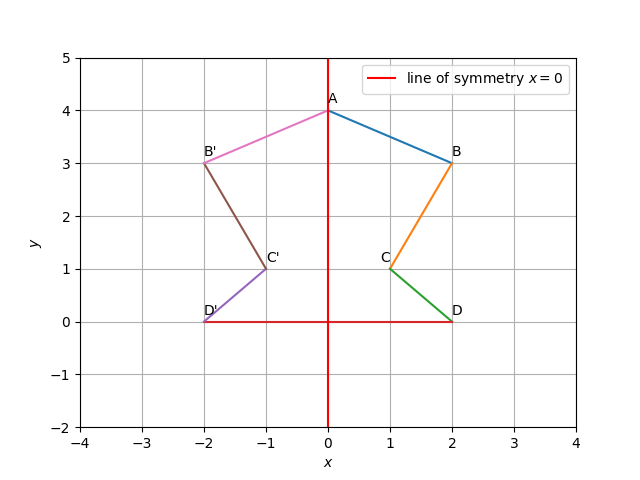
\includegraphics[scale=0.7]{./Figs/Figure_1.png}
 	  \caption{Plot of all points and figure formed}
 \end{figure}
\end{document}